%% PNAStmpl.tex
%% Template file to use for PNAS articles prepared in LaTeX
%% Version: Apr 14, 2008


%%%%%%%%%%%%%%%%%%%%%%%%%%%%%%
%% BASIC CLASS FILE
%% PNAStwo for two column articles is called by default.
%% Uncomment PNASone for single column articles. One column class
%% and style files are available upon request from pnas@nas.edu.
%% (uncomment means get rid of the '%' in front of the command)

%\documentclass{pnasone}
\documentclass{pnastwo}

%%%%%%%%%%%%%%%%%%%%%%%%%%%%%%
%% Changing position of text on physical page:
%% Since not all printers position
%% the printed page in the same place on the physical page,
%% you can change the position yourself here, if you need to:

% \advance\voffset -.5in % Minus dimension will raise the printed page on the
                         %  physical page; positive dimension will lower it.

%% You may set the dimension to the size that you need.

%%%%%%%%%%%%%%%%%%%%%%%%%%%%%%
%% OPTIONAL GRAPHICS STYLE FILE

%% Requires graphics style file (graphicx.sty), used for inserting
%% .eps files into LaTeX articles.
%% Note that inclusion of .eps files is for your reference only;
%% when submitting to PNAS please submit figures separately.

%% Type into the square brackets the name of the driver program
%% that you are using. If you don't know, try dvips, which is the
%% most common PC driver, or textures for the Mac. These are the options:

% [dvips], [xdvi], [dvipdf], [dvipdfm], [dvipdfmx], [pdftex], [dvipsone],
% [dviwindo], [emtex], [dviwin], [pctexps], [pctexwin], [pctexhp], [pctex32],
% [truetex], [tcidvi], [vtex], [oztex], [textures], [xetex]

%\usepackage[dvips]{graphicx}

%%%%%%%%%%%%%%%%%%%%%%%%%%%%%%
%% OPTIONAL POSTSCRIPT FONT FILES

%% PostScript font files: You may need to edit the PNASoneF.sty
%% or PNAStwoF.sty file to make the font names match those on your system.
%% Alternatively, you can leave the font style file commands commented out
%% and typeset your article using the default Computer Modern
%% fonts (recommended). If accepted, your article will be typeset
%% at PNAS using PostScript fonts.

% Choose PNASoneF for one column; PNAStwoF for two column:
%\usepackage{PNASoneF}
\usepackage{PNAStwoF}

%%%%%%%%%%%%%%%%%%%%%%%%%%%%%%
%% ADDITIONAL OPTIONAL STYLE FILES

%% The AMS math files are commonly used to gain access to useful features
%% like extended math fonts and math commands.

\usepackage{amssymb,amsfonts,amsmath}

%\usepackage{subcaption}
\graphicspath{ {paper_figures2/} }

%\usepackage{sansmath}

%\usepackage[font={sf, small}]{caption}

%%%%%%%%%%%%%%%%%%%%%%%%%%%%%%
%% OPTIONAL MACRO FILES
%% Insert self-defined macros here.
%% \newcommand definitions are recommended; \def definitions are supported

%\newcommand{\mfrac}[2]{\frac{\displaystyle #1}{\displaystyle #2}}
%\def\s{\sigma}

\DeclareMathSizes{9}{8}{7}{7}

\DeclareMathOperator*{\argmin}{arg\,min}

\makeatletter
\newcommand{\customlabel}[2]{%
\protected@write \@auxout {}{\string \newlabel {#1}{{#2}{}}}}
\makeatother

%%%%%%%%%%%%%%%%%%%%%%%%%%%%%%
%% Don't type in anything in the following section:
%%%%%%%%%%%%
%% For PNAS Only:
\contributor{Submitted to Proceedings
of the National Academy of Sciences of the United States of America}
\url{www.pnas.org/cgi/doi/10.1073/pnas.0709640104}
\copyrightyear{2008}
\issuedate{Issue Date}
\volume{Volume}
\issuenumber{Issue Number}
%%%%%%%%%%%%

\begin{document}

%%%%%%%%%%%%%%%%%%%%%%%%%%%%%%


%% For titles, only capitalize the first letter
%% \title{Almost sharp fronts for the surface quasi-geostrophic equation}

\title{Temporal ordering and registration of cross-sectional imaging data}


%% Enter authors via the \author command.
%% Use \affil to define affiliations.
%% (Leave no spaces between author name and \affil command)

%% Note that the \thanks{} command has been disabled in favor of
%% a generic, reserved space for PNAS publication footnotes.

%% \author{<author name>
%% \affil{<number>}{<Institution>}} One number for each institution.
%% The same number should be used for authors that
%% are affiliated with the same institution, after the first time
%% only the number is needed, ie, \affil{number}{text}, \affil{number}{}
%% Then, before last author ...
%% \and
%% \author{<author name>
%% \affil{<number>}{}}

%% For example, assuming Garcia and Sonnery are both affiliated with
%% Universidad de Murcia:
%% \author{Roberta Graff\affil{1}{University of Cambridge, Cambridge,
%% United Kingdom},
%% Javier de Ruiz Garcia\affil{2}{Universidad de Murcia, Bioquimica y Biologia
%% Molecular, Murcia, Spain}, \and Franklin Sonnery\affil{2}{}}

\author{Carmeline~J.~Dsilva\affil{1}{Department of Chemical and Biological Engineering, Princeton University, Princeton, New Jersey, USA},
Bomyi~Lim\affil{1}{},
Thomas~J.~Levario\affil{2}{School of Chemical and Biomolecular Engineering, Georgia Institute of Technology, Atlanta, Georgia, USA},
Hang~Lu\affil{2}{},
Amit~Singer\affil{3}{Department of Mathematics, Princeton University, Princeton, New Jersey, USA} \affil{4}{Program in Applied and Computational Mathematics, Princeton University, Princeton, New Jersey, USA},
Stanislav~Y.~Shvartsman\affil{1}{} \affil{5}{Lewis-Sigler Institute for Integrative Genomics, Princeton University, Princeton, New Jersey, USA},
\and
Ioannis~G.~Kevrekidis\affil{1}{} \affil{4}{Program in Applied and Computational Mathematics, Princeton University, Princeton, New Jersey, USA}}

\contributor{Submitted to Proceedings of the National Academy of Sciences
of the United States of America}

%% The \maketitle command is necessary to build the title page.
\maketitle

%%%%%%%%%%%%%%%%%%%%%%%%%%%%%%%%%%%%%%%%%%%%%%%%%%%%%%%%%%%%%%%%
\begin{article}

\begin{abstract}
In studies of development, researchers are often presented with cross-sectional data, where each data point is a sample from a population fixed at a slightly different developmental time.
%
The goal is then to temporally order the data to reconstruct the developmental dynamics.
%
If each data point is a two-dimensional image, the images must first be registered before they can be temporally ordered.
%
When such data sets are large, noisy, and/or if the developmental changes are subtle, these tasks can be difficult to do by hand.
%
We present an automatic approach to register {\it and} temporally order cross-sectional data sets of images.
%
The mathematical techniques (vector diffusion maps) are applicable to a wide variety of data sets and
require little {\it a priori} knowledge of the image features or the developmental dynamics.
%
We demonstrate the utility of these methods using a collection of images from a study of {\it Drosophila} embryogenesis.
\end{abstract}


%% When adding keywords, separate each term with a straight line: |
\keywords{temporal ordering | image registration}

%% Optional for entering abbreviations, separate the abbreviation from
%% its definition with a comma, separate each pair with a semicolon:
%% for example:
%% \abbreviations{SAM, self-assembled monolayer; OTS,
%% octadecyltrichlorosilane}

% \abbreviations{}

%% The first letter of the article should be drop cap: \dropcap{}
%\dropcap{I}n this article we study the evolution of ''almost-sharp'' fronts

%% Enter the text of your article beginning here and ending before
%% \begin{acknowledgements}
%% Section head commands for your reference:
%% \section{}
%% \subsection{}
%% \subsubsection{}



\dropcap{E}xperimental studies of developmental dynamics fall in two broadly defined categories: longitudinal and cross-sectional \cite{diggle2002analysis}.
%
In longitudinal studies, developmental progress is monitored over time for the same embryo.
%
In a cross-sectional study, developmental dynamics must be reconstructed from multiple snapshots of different embryos, each of which contributes only a single snapshot of a chemical or morphological process along its developmental trajectory.
%
Both of these sampling schemes have their advantages and limitations, and both are extensively used by biologists.
%
Here we focus on cross-sectional studies, which have a time-honored history and still present the only option for most organisms.
%
In a typical cross-sectional study, a group of developing embryos is fixed using a procedure that arrests their development and stained with chemicals that visualize a handful of cellular processes.
%
Fixed embryos are then imaged using any given number of microscopy techniques.
%
Recent advances in large-scale physical manipulation and imaging of embryos produce rapidly increasing volumes of cross-sectional data, in which every embryo is observed at a different geometric orientation and developmental time point.
%
Importantly, the ``age'' of any given embryo arrested in its development is not known to high accuracy.
%
In general, it is only known that a collection of embryos belongs to a certain time window.
%
In order to recover the developmental dynamics from such datasets, snapshots of different embryos must be spatially aligned or registered to factor out the relevant symmetries (i.e., translations and rotations), and then ordered in time.
%
We show how existing dimensionality reduction algorithms can greatly accelerate {\it and combine} both of these tasks.

Temporal ordering and registration of images is straightforward when the number of images is small and differences between them are visually apparent.
%
As an example, Figure~\ref{fig:fish} shows a caricature of fish development which illustrates the processes of growth and patterning.
%
In this case, temporal ordering can be accomplished by arranging the fish by size, which is monotonic with the developmental progress.
%
Image registration is based on obvious morphological landmarks, such as the position of head and fins.
%
In contrast to this simple illustration, real data poses nontrivial challenges for both registration and temporal ordering. 
%
In general, the landmarks needed for registration, such as the heads and fins in our example, as well as the features that can be used to order the data, such as the body length, are not known {\it a priori}.
%
Additional challenges arise from embryo-to-embryo variability, sample size, and measurement noise. 

\begin{figure}[t]
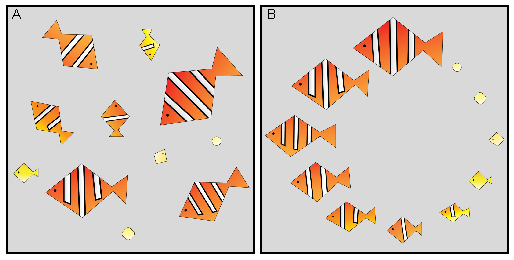
\includegraphics[width=8.4cm]{fig1}
\caption{{\it (A)} Fish, each in a different orientation and a different stage of development. {\it (B)} Fish, now rotationally registered and temporally ordered. For this caricature, the registration and ordering is easy to do ``by hand" because the data set is small and the developmental changes are easy to recognize.}
%\label{fig:fish}
\customlabel{fig:fish}{1}
\customlabel{subfig:fish_unordered}{\ref{fig:fish}{\it A}}
\customlabel{subfig:fish_ordered}{\ref{fig:fish}{\it B}}
\end{figure}

Here, we show how recently developed dimensionality reduction techniques can successfully address these challenges and reveal developmental trajectories from collections of unregistered and unordered imaging data. 
%
We will demonstrate these techniques using two data sets from a study of {\it Dropophila} embryogenesis.
%
The first data set, shown in Figure~\ref{subfig:raw_data1}, is relatively simple and will allow us to both illustrate and validate our methods. 
%
In the second data set, shown in Figure~\ref{subfig:raw_data2}, the dynamics are significantly more complex; here, we will show that we can recover a trajectory that is qualitatively consistent with current knowledge.


%\begin{itemize}
%\item Imaging data is becoming increasingly prevalent in biology research.
%
%\item General motivation about biology data ...
%
%\item Need methods to organize data, visualize, ...
%
%\item REDUCTION is important, reduction because of symmetry and reduction because of content
%
%\item There are a bunch of recent techniques- some established (like dmaps), some very fresh, like synchronization or VDMaps,  that have had their own reasons to be developed but they are as if tailor made for what we would want to do
%\end{itemize}


\section{Results and Discussion}

\subsection{Vector diffusion maps for registration and temporal ordering}

A typical dataset from cross-sectional studies of developmental processes is a collection of images of different embryos, each of which is fixed at a different developmental time and imaged in a different rotational orientation.
%
We would like to organize these data sets in a meaningful and informative way.
%
This requires rotating and translating each image so the set is in a consistent frame of reference ({\it registration}), and then temporally ordering the images. 
%
We will show that dimensionality reduction algorithms can accomplish both of these tasks and therefore give us a meaningful picture of the underlying developmental dynamics. 

Our approach is based on vector diffusion maps \cite{singer2012vector}, a general technique developed for data sets which contain two sources of variability:
symmetries (such as translations and rotations of the images due to the imaging setup) which one would like to factor out, and other directions of variability (such as temporal dynamics) which one would like to uncover.
%
Vector diffusion maps combine two algorithms, angular synchronization \cite{singer2011angular} for image registration and diffusion maps \cite{coifman2005geometric} for extracting low-dimensional structure, into one computation that allows us to simultaneously register and temporally order our images. 
%
Vector diffusion maps has been applied to cryo-EM images \cite{...}, where each image is a projection of a molecule, taken from a different viewing direction and in a different rotation. 
%
Here, we will use the algorithm to register images of {\it Drosophila} embryos with respect to rotations and translations to remove variability from the imaging procedure, as well as uncover the main direction of variability {\it after} removing translational and rotational symmetries.
%
We assume that, in this set of images, this main direction of variability is parameterized by time. 
%
Unlike the noise in the cryo-EM application, which is approximately Gaussian, the noise in our experiments is primarily from interembryo variability and does not have a known simple structure.

Registration via angular synchronization/vector diffusion maps uses pairwise alignment information to register the set of images in a globally consistent way.
%
A schematic illustration is shown in Figure~\ref{subfig:synch1}; each image is depicted as a vector, and the goal is to align the set of vectors. 
%
We first compute the angles needed to align pairs of vectors (or images).
%
In general, this requires no template function or image landmarks; however, when the images are noisy, some pairwise alignment angles may be inaccurate.
%
Using the angles between all pairs of vectors (or images), angular synchronization/vector diffusion maps then finds the set of rotation angles, one angle for each vector (or image), that is most consistent with the pairwise measurements. 
%
In this schematic, registration via angular synchronization is trivial as the pairwise measurements contain no noise. 
%
Angular synchronization/vector diffusion maps can successfully register sets of vectors (or images) even when many of the pairwise measurements are corrupted by noise. 
%

%
After removing the variability due to translations and rotations of the images, the remaining variability arises (mostly) due to developmental dynamics.
% 
These dynamics can be revealed by ordering the data along a one-dimensional manifold that parametrizes the data. 
%
Such a manifold can be discovered using diffusion maps \cite{coifman2005geometric}, a nonlinear dimensionality reduction technique;
this algorithm uncovers a parameterization of data that lies on a low-dimensional, perhaps nonlinear, manifold in high-dimensional space. 
%
This idea is illustrated in Figure~\ref{subfig:dmaps1}: the data are two-dimensional points which lie on a one-dimensional nonlinear curve. 
%
We use {\it local} information about the data to find a ``good'' parameterization: we want points which are close in high-dimensional space (i.e., images which look similar) to be close in our parameterization.
%
This idea of locality is illustrated by the edges in Figure~\ref{subfig:dmaps1}; data points which are close are connected by dark edges, and clearly, the dark edges are more informative about the low-dimensional structure of the data. 
%
The color in Figure~\ref{subfig:dmaps2} depicts the one-dimensional parameterization or ordering of the data that we can detect visually.
%
In our examples, each data point will be very high dimensional (e.g, an image with many pixels), and so we cannot extract this low-dimensional structure visually.
%
Instead, we will rely on diffusion maps to automatically extract a parameterization of our high-dimensional data.
%
We will assume that our data are approximately one-dimensional, and that this dimension is parameterized by time, such that ordering our data along this main dimension/direction will temporally order our data. 

Both angular synchronization and diffusion maps use pairwise information to extract a global structure in the data.
%
Angular synchronization uses pairwise alignment information to find translations and rotations which are globally consistent, and diffusion maps uses pairwise distances to find parameterizations which are globally informative.
%
Vector diffusion maps combines both steps into one computation;
the algorithm uses information about pairwise alignments and pairwise distances to find a global parameterization of the data, while registering images which are ``close''.
%
The algorithm is ``tailor-made'' for our task of registering and temporally ordering cross-sectional imaging data; we will use it to uncover a temporal ordering of our images, as well as register images which are developmentally similar, to obtain a global picture of development.

\begin{figure}[t]
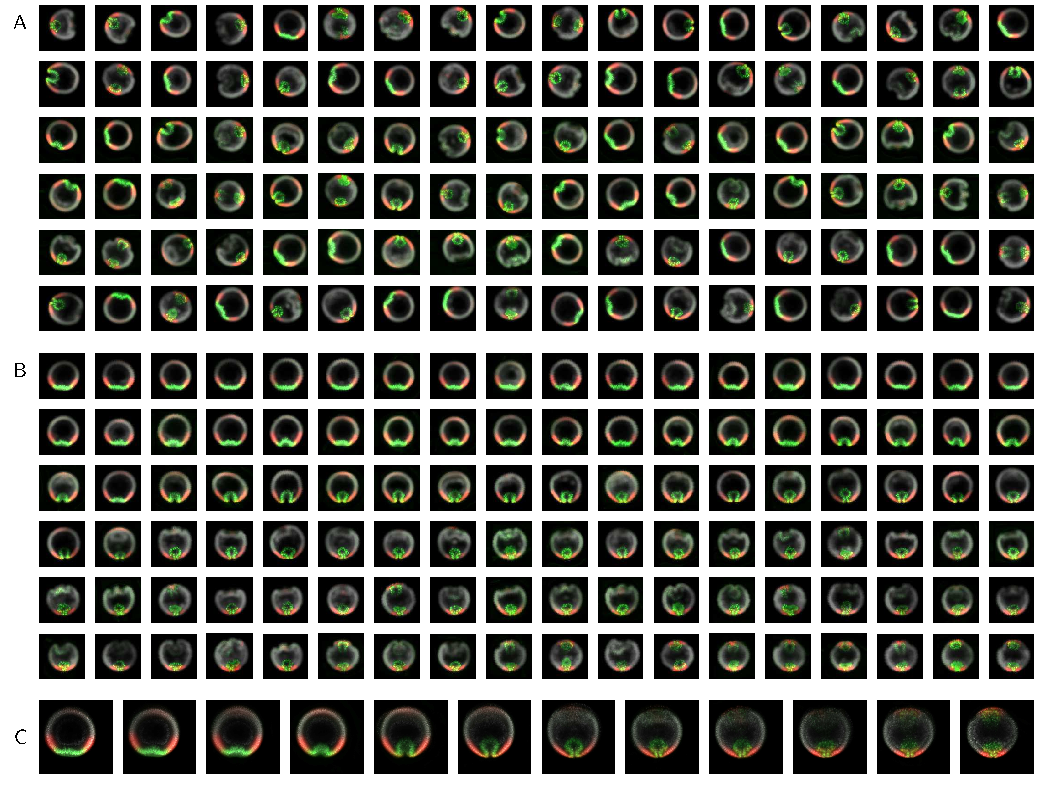
\includegraphics[width=8.4cm]{fig4}
\caption{ {\it (A)} Set of vectors, each in a different orientation. The pairwise alignment angles are indicated. {\it (B)} The vectors from {\it A}, each rotated so that the set is globally aligned. Note that the chosen rotation angles are consistent with the pairwise alignments in {\it A}. {\it (C)} Data points (in black) which lie on a one-dimensional nonlinear curve in two dimensions. Each pair of data points is connected by an edge, and the edge weight is related to the Euclidean distance between the points through the diffusion kernel (see {\it SI Appendix}), so that close data points are connected by dark (``stronger'') edges. {\it (D)} The data in {\it C}, colored by the first (non-trivial) eigenvector from the diffusion map computational procedure, $\phi_2$. The color intensity is monotonic with the arclength, thus parameterizing the curve.}
%\label{fig:schematics}
\customlabel{fig:schematics}{2}
\customlabel{subfig:synch1}{\ref{fig:schematics}{\it A}}
\customlabel{subfig:synch2}{\ref{fig:schematics}{\it B}}
\customlabel{subfig:dmaps1}{\ref{fig:schematics}{\it C}}
\customlabel{subfig:dmaps2}{\ref{fig:schematics}{\it D}}
\end{figure}


\subsection{Images of {\it Drosophila} embryos during cellularization}

%
As a first illustration of this approach to temporal ordering and registration of images, we used a dataset where the correct registration and temporal order is known. 
%
This dataset is obtained by fluorescent imaging of {\it Drosophila} embryos during the third hour after fertilization.
%
By this stage of development, sequential divisions of the fertilized egg have generated a system where most of the nuclei are arranged in a monolayer under the common plasma membrane.
%
Figure 3a shows optical cross-sections of each embryo, with nuclei (gray) labelled by a DNA stain. 
%
The spatially uniform arrangement of nuclei is patterned by the concentration profiles of chemical signals that act as dose-dependent regulators of cell differentiation.
%
One of these signals is provided by the nuclear localization of transcription factor Dorsal (Dl, green), which subdivides the embryo into the territories that give rise to the muscle, nerve, and skin tissues.
%
Another signal is provided by the phosphorylated form of the extracellular signal regulated kinase (dpERK), an enzyme that specifies a subset of neuronal cells. 
%

Previous studies \cite{...} established that throughout the 3rd hour of development, the nuclear localization of Dl is unimodal and peaked at the ventral side of the embryo. 
%
The spatiotemporal pattern of dpERK is more complex: dpERK is first detected in two lateral stripes, which increase in intensity towards the end of the 3rd hour. 
%
This bimodal pattern is then augmented by a peak at the dorsal side of the embryo.
%
Both of these features become readily apparent when images are registered and ordered using vector diffusion maps: the peak of nuclar Dl is consistent throughout the images and intensity of the dpERK signal in the lateral regions of the embryo monotonically increases across the dataset.
%
The quality of the temporal ordering provided by vector diffusion maps can be assessed by comparing with the temporal ordering provided by an independent approach.
%
Specifically, during this developmental timespan, the embryo cellularizes: nuclei located under common plasma membrane are enclosed by lateral membranes which grow inward, separating nuclei into individual cells.
%
The highly reproducible kinetics of lateral membrane growth can be used to estimate the age of each embryo within 1-3 minutes  \cite{...} (see {\it SI Appendix}).    
%
The rank correlation coefficient between the orderings provided by membranes and vector diffusion maps is 0.9127. 
%
Thus, we have validated a dimensionality reduction approach to temporal ordering and registration of data  on a dataset where image orientation and ordering can be assessed independently. 

%Furthermore, the dynamics uncovered by vector diffusion maps is relatively simple, which suggests that a simpler approach could have been used to order the data.
%
%Indeed, a principal component analysis (PCA) of registered data reveals that data can be accurately ordered by projecting each image onto the first PCA mode. 


\begin{figure*}[t]
\raisebox{8.1cm}{{\figtextfont A}}
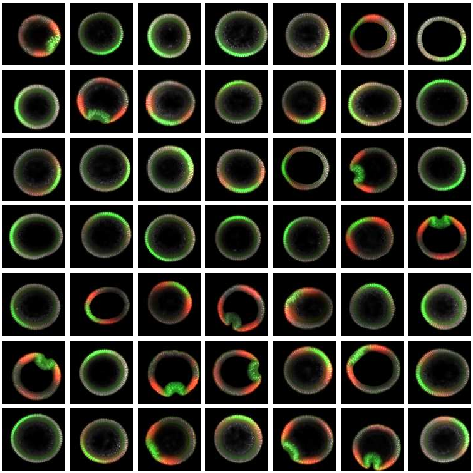
\includegraphics[width=8.4cm]{raw_data1}
\hfill
\raisebox{8.1cm}{{\figtextfont B}}
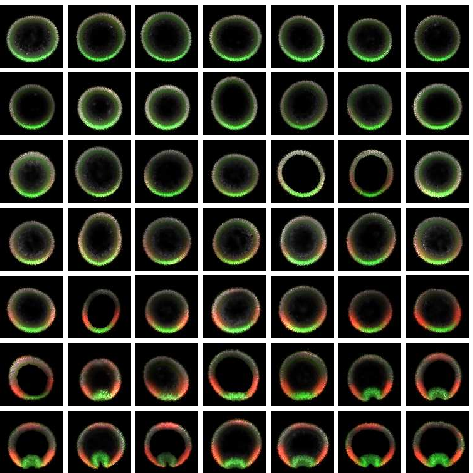
\includegraphics[width=8.4cm]{VDM_data1_ordered}\\
%\vspace{0.2cm}
%\centering
%\raisebox{0.5cm}{{\figtextfont C}}
%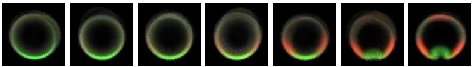
\includegraphics[width=8.4cm]{average_trajectory_VDM}
\caption{{\it (A)} Images of {\it Drosophila} embryos during cellularization. Each image is of a different embryo in a different rotational orientation. {\it (B)} Images from {\it A}, now registered and ordered using vector diffusion maps. }%{\it (C)} Average trajectory of the images shown in {\it B}.  Each image is the average of $7$ consecutive images in {\it B}. }
\customlabel{fig:data1}{3}
\customlabel{subfig:raw_data1}{\ref{fig:data1}{\it A}}
\customlabel{subfig:ordered_data1}{\ref{fig:data1}{\it B}}
\customlabel{subfig:averaged_data1}{\ref{fig:data1}{\it C}}
\end{figure*}


\subsection{Images of gastrulating {\it Drosophila} embryos}

Because the images in Figure~\ref{fig:data1} are relatively simple, simpler techniques could have been used to temporally order this particular data set. 
%
Because these data are effectively a single mode (the two lateral dpERK peaks) growing in time,
principal component analysis \cite{shlens2005tutorial} would uncover most of the meaningful structure in the data, and projection onto the first principal component would be sufficient to order the data.
%
However, developmental dynamics are often significantly more complex, and nonlinear techniques such as diffusion maps/vector diffusion maps are required to extract meaningful structure in the data. 
%
Figure~\ref{subfig:raw_data2} shows a data set of $108$ images of {\it Drosophila} embryos;
these images cover a thirty minute time interval and span late cellularization through gastrulation, when tissues within the embryo begin to morph and deform. 
%
Each image shows the optical cross-section of an embryo fixed at a different developmental time.
%
The nuclei (gray) are again labeled with a DNA marker.
%
However, during this developmental time period, and the nuclei are no longer uniformly arranged around the periphery of the embryo, as the tissue begins to deform and morph.
%
Twist (Twi, shown in green) denotes the ventralmost point of the embryo (similar to Dl in the previous data set); during this developmental time span, the ventral furrow is formed, where the ventral side invaginates towards the center of the embryo.
%
dpERK (red) again appears as two lateral peaks at the ventral side of the embryo.
%
These two peaks merge together during invagination, eventually forming (together with Twi) a characteristic ``omega'' shape.
%
During this developmental timespan, germ band elongation causes cells from the ventral side of the embryo to move towards the poles, and then wrap around to the dorsal side of the embryo.
%
At the end of this developmental timespan, cells which were originally on the ventral side of the embryo have migrated to the dorsal side of the embryo, causing similar ``omega'' shaped patterns (formed by Twi and dpERK) to arise on the dorsal side.
%
Although we know about this general developmental progression, unlike the previous data set, we have no independent way to measure the precise developmental time of each embryo.
%
We are forced to use other methods to temporally order these images.

The dynamics in this data set are highly nonlinear, and only 22\% of the variability in the data is captured by the first principal component.
%
We require a more sophisticated approach, such as vector diffusion maps, to temporally order the data.
%
Figure~\ref{subfig:ordered_data2} shows the images in Figure~\ref{subfig:raw_data2}, now registered and ordered using vector diffusion maps \cite{singer2012vector}.
%
The ordering is consistent with the known developmental dynamics outlined above.

However, because each image comes from a {\it different} embryo, the recovered trajectory is still noisy due to interembryo variability.
%
We would like to extract an average developmental trajectory from this set of registered and temporally ordered images to obtain a representative picture of the dynamics.
%
A simple method for doing this is dividing the ordered data set into groups or stages, and then computing the average image at each stage. 
%
Figure~\ref{sub fig:averaged_data2} shows the average trajectory for our data set, and it is now very straightforward to see the underlying developmental dynamics.

\newpage
\begin{figure*}[t]
\raisebox{5.3cm}{{\figtextfont A}}
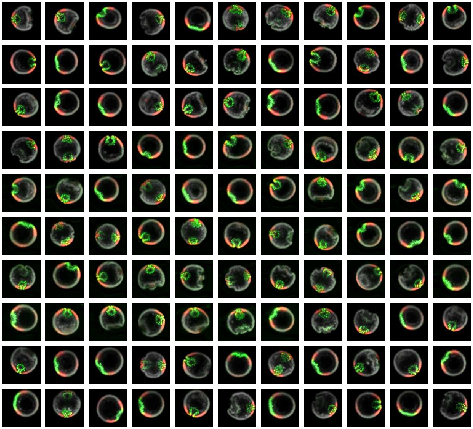
\includegraphics[width=16.8cm]{raw_data2}

\vspace{0.2cm}
\raisebox{5.3cm}{{\figtextfont B}}
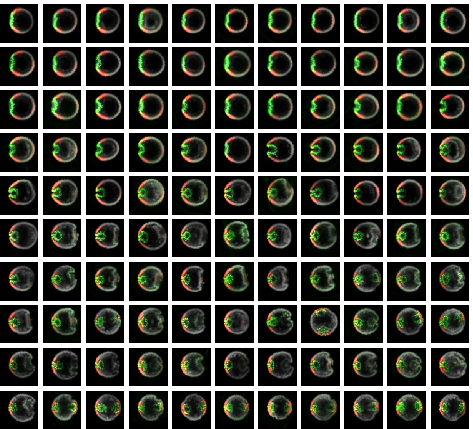
\includegraphics[width=16.8cm]{VDM_ordered}

\vspace{0.2cm}
\raisebox{0.6cm}{{\figtextfont C}}
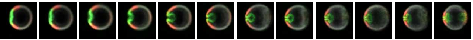
\includegraphics[width=16.8cm]{average_trajectory}
\caption{{\it (A)} Images of gastrulating {\it Drosophila} embryos. Each image is of a different embryo in a different rotational orientation. {\it(B)} Data from {\it A}, registered and ordered using vector diffusion maps. {\it (C)} Average trajectory of the images shown in {\it B}. Each image is the average of $9$ consecutive images in {\it B}. }
\customlabel{fig:data2}{4}
\customlabel{subfig:raw_data2}{\ref{fig:data2}{\it A}}
\customlabel{subfig:ordered_data2}{\ref{fig:data2}{\it B}}
\customlabel{subfig:averaged_data2}{\ref{fig:data2}{\it C}}
\end{figure*}

\section{Conclusions}

We have demonstrated how vector diffusion maps, an existing reduction technique, can be used to register and temporally order images from developmental biology studies. 
%
We acknowledge that the tasks of both registration and ordering can be accomplished using a variety of techniques.
%
We chose the techniques outlined here, not because they are specifically tailored to our particular data sets, but rather, because they are sufficiently general and we are confident that they can be applied to a myriad of biological imaging applications. 

The task of image registration has been widely studied \cite{zitova2003image}, for applications such as face recognition \cite{rowley1998rotation}, medical image registration \cite{hajnal2010medical}, and texture classification \cite{greenspan1994rotation}.
%
However, most of these applications rely on the definition and identification of good {\it features} within each image. 
%
For example, in face recognition, the first step is often to find the eyes, nose, and mouth within the face, and then register images by aligning these features \cite{zhao2003face}.
%
%Temporally ordering images of a construction site over time is also based on first identifying features within the images \cite{schindler2007inferring}.
%
For our biological applications, good features may not be known {\it a priori}.
%
We instead use an algorithm which requires no features, but instead, uses only the raw pixel images and the inherent geometric symmetry of the problem.
%
%Template-based methods are also common for registration, where one optimally aligns each image to a predefined template function.
%
%However, these methods can suffer when the images are noisy, and the success of such methods can depend strongly on the template function \cite{shatsky2009method}.
%

The task of temporal ordering has also been studied in a variety of biological applications. 
%
Data sets such as  RNA sequencing data \cite{anavy2014blind, trapnell2014dynamics} (where each data point is the transcriptome for a single sample), gene expression data from multiple patients \cite{gupta2008extracting, qiu2011discovering} (where each data point is a vector containing the expression levels of the various genes), and snapshots of cells throughout the cell cycle (where each point is a vector of features, e.g., amount of DNA which quantify the cell's state)  \cite{kafri2013dynamics} have all been temporally ordered to extract the trajectory of the underlying dynamic process.
%
Most of these applications order the data by solving a traveling salesman problem or constructing a minimum spanning tree on the data,
expecting that these structures (the path of the traveling salesman, or the minimum spanning tree) characterize the majority of the structure/variability within the data and provide an accurate encoding of the dynamical progression.
%
Furthermore, many of these algorithms use PCA (a dimensionality reduction technique) as an initial preprocessing/denoising step. 
%
We, instead, use vector diffusion maps to construct a one-dimensional parameterization of the data.
%
Because vector diffusion maps is a dimensionality reduction technique, it acts as a denoising step (as indicated by the smoothness of our averaged trajectories).
%
However, because it is nonlinear, it affords us many of the same geometric flexibilies as the MST or TSP formulations. 
%
Vector diffusion maps are one of many nonlinear dimensionality reduction techniques that have been recently developed \cite{Belkin2003, tenenbaum2000global, Donoho2003, Roweis2000}.
%
They have been shown to be more robust to noise than other path-based algorithms, such as isomap \cite{balasubramanian2002isomap}, and so we suspect they may perform better than the ordering algorithms used in previous work.

Furthermore, dimensionality reduction techniques such as vector diffusion maps do not constrain us to one-dimensional parameterizations/organizations of the data.
%
For this particular application, we expect our data to be one-dimensional, as the only (main) source of variability is time.
%
However, other sources of variability, such as size, viewing angle, and mutation state, could also be uncovered using vector diffusion maps.
%
We could therefore use these same algorithms for tasks such as classification of embryos by size or viewing angle, and comparison of the developmental dynamics in different mutations.

After registering and temporally ordering images, one can perform a variety of post-processing tasks to gain further insight into the developmental processes.
%
We have demonstrated one post-processing technique (window averaging) that allows us to extract a more representative developmental trajectory from the set of noisy snapshots. 
%
However, tasks such as constructing a smooth movie from these cross-sectional snapshots would also be of biological interest.
%
One could look not only at the window averages, but also at the top principal components in each window to see the main dynamical features along the trajectory.
%
All of these questions first require that the data be registered and temporally ordered.
%
We are confident that, as imaging becomes easier and more robust, the techniques we present here will play an important role in the data analysis pipeline. 


%\begin{itemize}
%\item What are other people doing  (maybe critically)
%\item Movies  smoothness
%\item Discrete symmetries like flips
%\item Local information ? (features of the image) (associate with Fourier-Bessel and bispectra)
%\item Mutant-wildtype stuff  IMPORTANT
%\item And in general, MULTIPLE variablities is important (mutants, guys in another cycle, etc.)
 
%\item size is an issue
%\item  small tilts is an issue
%\item   could one do three-d image processing ?  of the floating thing, without the device
%\item how do we go about merging datasets ?
%\end{itemize}



\bibliographystyle{pnas}
\bibliography{background_reading/references,../../references/references}

\end{article}

\end{document}

